\documentclass[11pt,a4paper]{article}
\usepackage[utf8]{inputenc}
\usepackage[T1]{fontenc}
\usepackage[brazil]{babel}
\usepackage{lmodern}
\usepackage[margin=2cm]{geometry}
\usepackage{amsmath,amssymb,bm}
\usepackage{graphicx}
\usepackage{booktabs}
\usepackage{float}
\usepackage[hidelinks]{hyperref}
\title{Plano de trabalho: etapas 1, 2 e 3\\\large SRM corrigido, FORM e amostragem por importância no Cho (2010)}
\date{16/11/2026}
\begin{document}
\maketitle

\section*{Resumo}
\begin{itemize}
  \item \textbf{SRM corrigido (etapa 1):} começar o caminho de $F$ em 0,8, e não em 1, quase não muda a $P_f$.
    No Cho2010, as falhas são as mesmas nas 1000 realizações pareadas. Na chuva, 4 realizações passam a falhar e 1 deixa de falhar (McNemar $p = 0{,}38$).
  \item \textbf{AI contra o direto (etapas 2 e 3):} todas as AI concordam com o Monte Carlo direto do mesmo modelo, a menos de
    1,3 desvio. O ganho cresce quando a $P_f$ cai: até 16$\times$ com
    $P_f \approx 1{,}7\,\%$ e até 51$\times$ com $P_f \approx 0{,}4\,\%$.
    O melhor deslocamento é o ponto de projeto do FORM com $M = 20$.
  \item \textbf{FORM sozinho:} com $M = 10$ ele acerta por coincidência, e com $M = 20$ superestima a $P_f$ em 30 a 45\,\%.
    Ele é bom para escolher o deslocamento da AI, mas não serve como estimativa final.
  \item \textbf{Um modo de ruptura só:} todas as falhas do direto estão do lado do ponto de projeto ($t = \bm\alpha\cdot\bm\xi \ge 1{,}3$), e a banda de ruptura é a mesma no direto e na AI. A AI pelo
    FORM não está perdendo falhas.
\end{itemize}

\section{O que rodou}
Tudo rodou no fermi, nas campanhas \texttt{etapa1} (15/11) e \texttt{etapa3} (noite de 15 para 16/11), com o SRM novo,
tri2 + 4 níveis e a KL analítica de 2000 termos por campo. O problema é o talude seco do Cho (2010), Exemplo 2: $c'$ com média
10\,kPa e CoV 0,3; $\varphi'$ com média $30^\circ$ e CoV 0,2; campos lognormais com $l_h = 20$\,m e $l_v = 2$\,m; correlação
cruzada $r = -0{,}5$ ou $-0{,}7$. O FS determinístico é 1,2044, contra 1,204 do Cho.

\section{Etapa 1: o SRM corrigido}
\begin{itemize}
  \item \textbf{O defeito:} com $F_0 = 1$, o peso às vezes convergia num talude com FS logo abaixo de 1, e o FS saía $\ge 1$.
    Na campanha antiga dos solos (f50, todos os instantes), há 13 FS em $[0{,}995;\,1)$ e 47 em $[1;\,1{,}005)$, e nenhum em $[0{,}999;\,1)$.
  \item \textbf{O teste:} as mesmas realizações com as duas versões, na mesma máquina e com as mesmas opções.
\end{itemize}
\begin{table}[H]\centering\small
\resizebox{\textwidth}{!}{%
\begin{tabular}{lrrrrrrr}
\toprule
Caso & pares & falhas antigo & falhas novo & passam a falhar & deixam & McNemar $p$ & dif. FS: média (dp) \\
\midrule
Cho2010, $r = -0{,}5$ & 1000 & 22 & 22 & 0 & 0 & 1{,}00 & 0{,}00006 (0{,}0007) \\
chuva f50, 36 mm/h, 24 h & 600 & 137 & 140 & 4 & 1 & 0{,}38 & -0{,}00007 (0{,}0012) \\
\bottomrule
\end{tabular}}
\caption{SRM antigo contra o novo, realização a realização.}
\end{table}
\begin{figure}[H]\centering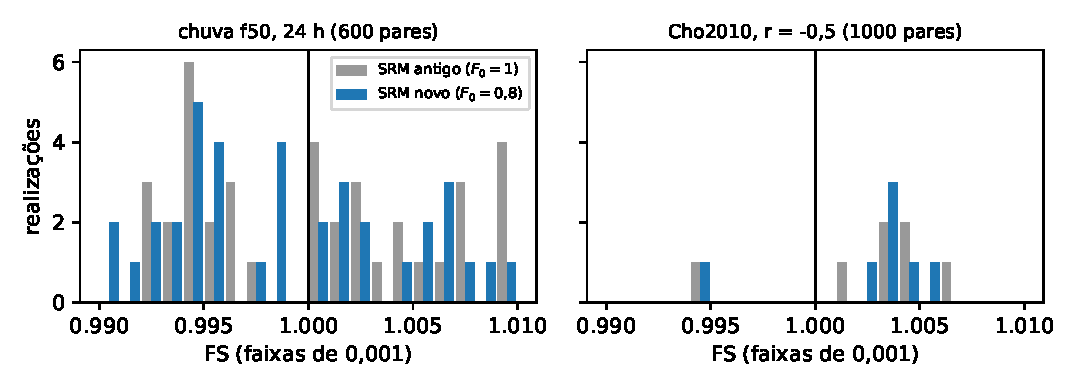
\includegraphics[width=\textwidth]{figs/srm_hist.pdf}
\caption{FS perto de 1 nas duas versões, nas mesmas realizações.}\end{figure}
\begin{itemize}
  \item \textbf{Efeito na $P_f$:} nulo no Cho2010 e de cerca de $+0{,}5$ ponto na chuva, onde a densidade de FS perto de 1 é
    maior.
  \item \textbf{Custo:} no Cho2010, perto de FS = 1, o fator novo leva 0{,}5 vezes o tempo do
    antigo (37 realizações); na média, 0{,}98 vezes. Na chuva, o novo foi
    mais rápido (0{,}57 vezes o tempo do antigo).
  \item \textbf{Decisão:} o SRM novo fica, porque é o correto.
  \item \textbf{Conferência de versão:} as 1000 primeiras realizações do direto com $r = -0{,}7$ rodaram duas vezes, com versões
    diferentes do programa (campanhas \texttt{etapa1} e \texttt{etapa3}). A maior diferença de FS foi 0{,}0000.
\end{itemize}

\section{Etapa 2: FORM e AI com $r = -0{,}5$ ($P_f \approx 1{,}7\,\%$)}
\begin{table}[H]\centering\small
\resizebox{\textwidth}{!}{%
\begin{tabular}{lrrrrrrr}
\toprule
Método & $N$ & $P_f$ (\%) & IC 95\% (\%) & CoV (\%) & dif. (desvios) & ESS$_F$ & ganho \\
\midrule
Monte Carlo direto & 24000 & 1{,}70 & 1{,}54–1{,}87 & 4{,}9 & --- & --- & 1 \\
AI pela banda (entropia cruzada) & 1000 & 1{,}74 & 1{,}36–2{,}12 & 11{,}1 & 0{,}2 & 75 & 4{,}6 \\
AI pelo FORM $M = 10$ & 1000 & 1{,}54 & 1{,}27–1{,}80 & 8{,}8 & -1{,}0 & 115 & 8{,}3 \\
AI pelo FORM $M = 20$ & 1000 & 1{,}53 & 1{,}35–1{,}72 & 6{,}3 & -1{,}3 & 202 & 16{,}2 \\
AI pelo FORM $M = 20$, semente 4 & 1000 & 1{,}72 & 1{,}52–1{,}92 & 5{,}9 & 0{,}2 & 222 & 16{,}3 \\
AI pelo FORM $M = 20$, semente 5 & 1000 & 1{,}90 & 1{,}67–2{,}12 & 6{,}1 & 1{,}4 & 214 & 14{,}1 \\
FORM, $M = 10$ ($\beta = 2{,}115$) & 123 análises & 1{,}72 & --- & --- & --- & --- & --- \\
FORM, $M = 20$ ($\beta = 2{,}012$) & 243 análises & 2{,}21 & --- & --- & --- & --- & --- \\
\bottomrule
\end{tabular}}
\caption{$r = -0{,}5$. Cho (2010): $P_f = 1{,}71\,\%$ (Monte Carlo de 50\,000, equilíbrio limite). dif.: a diferença AI $-$
direto em desvios-padrão. ESS$_F = (\sum w I)^2/\sum (wI)^2$. Ganho: quantas realizações do direto valem uma da AI, para
o mesmo CoV. O FORM com $M = 10$ e $M = 20$ convergiu em 3 iterações.}
\end{table}
\begin{figure}[H]\centering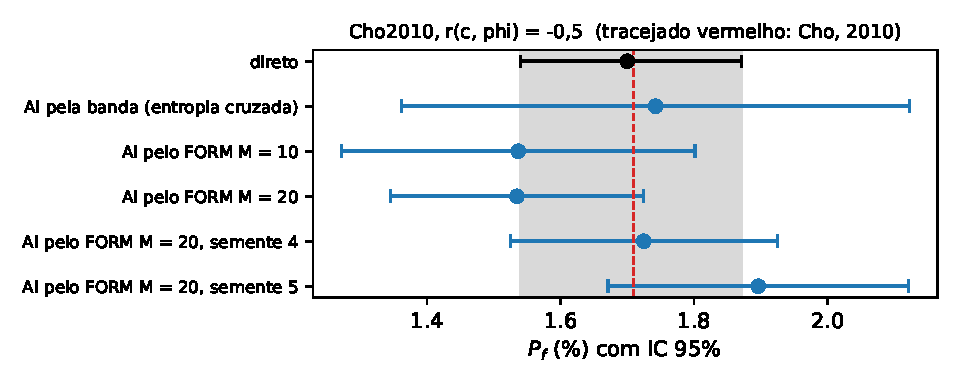
\includegraphics[width=0.85\textwidth]{figs/pf_r05.pdf}
\caption{$P_f$ e IC 95\,\%. A faixa cinza é o IC do direto; a linha tracejada, o valor do Cho.}\end{figure}

\paragraph{O teste linear (sem elementos finitos).}
O Cho2010 sorteia os campos como sempre, com a mesma semente, o mesmo deslocamento e o mesmo peso, mas troca o FS por
$\exp(\beta - \bm\alpha\cdot\bm\xi)$. A falha é $\bm\alpha\cdot\bm\xi > \beta$, com $P_f = \Phi(-\beta)$ exata. A direção
$\bm\alpha$ é a do ponto de projeto do FORM com $M = 20$. A AI ``M = 20'' desloca exatamente nessa direção. A AI ``M = 10'' usa
a direção do FORM com $M = 10$, a 17{,}6$^\circ$ da correta. Cada AI tem
$10^4$ realizações, e o direto, $10^6$.
\begin{table}[H]\centering\small
\resizebox{\textwidth}{!}{%
\begin{tabular}{rrrrr}
\toprule
$\beta$ & $P_f$ exata & direto ($10^6$) & AI $M = 20$: erro (desvios) & AI $M = 10$: erro (desvios) \\
\midrule
2 & 2.275e-02 & 2{,}27\,\% & 0{,}8\,\% (0{,}5) & -2{,}9\,\% (-1{,}6) \\
3 & 1.350e-03 & 0{,}13\,\% & 0{,}9\,\% (0{,}5) & -4{,}7\,\% (-1{,}7) \\
4 & 3.167e-05 & --- & 1{,}0\,\% (0{,}4) & -9{,}1\,\% (-2{,}6) \\
\bottomrule
\end{tabular}}
\caption{O teste linear.}
\end{table}
\begin{itemize}
  \item \textbf{O código da AI está certo:} com o deslocamento na direção exata, o erro fica abaixo de 1\,\% até
    $P_f = 3\times10^{-5}$.
  \item \textbf{Com o deslocamento um pouco fora da direção, a AI sai baixa,} e mais baixa quando $P_f$ cai. O estimador
    não tem viés, mas a região que mais pesa fica na cauda do sorteio: poucas amostras, com pesos enormes. Com $N$ finito,
    a estimativa típica fica abaixo do valor certo, e o CoV calculado subestima o erro.
  \item Isso explica a AI pelo FORM um pouco abaixo do direto no elementos finitos (Tabelas 2 e 3): o ponto de projeto
    nunca está exatamente na direção ótima.
\end{itemize}

\section{Etapa 3: $P_f$ pequena, $r = -0{,}7$ ($P_f \approx 0{,}4\,\%$)}
\begin{table}[H]\centering\small
\resizebox{\textwidth}{!}{%
\begin{tabular}{lrrrrrrr}
\toprule
Método & $N$ & $P_f$ (\%) & IC 95\% (\%) & CoV (\%) & dif. (desvios) & ESS$_F$ & ganho \\
\midrule
Monte Carlo direto & 25000 & 0{,}37 & 0{,}30–0{,}46 & 10{,}4 & --- & --- & 1 \\
AI pela banda (entropia cruzada) & 1000 & 0{,}45 & 0{,}31–0{,}59 & 16{,}3 & 0{,}9 & 36 & 8{,}4 \\
AI pelo FORM $M = 10$ & 1000 & 0{,}31 & 0{,}24–0{,}38 & 11{,}6 & -1{,}1 & 69 & 23{,}5 \\
AI pelo FORM $M = 20$ & 1000 & 0{,}35 & 0{,}29–0{,}41 & 8{,}6 & -0{,}4 & 119 & 38{,}3 \\
AI pelo FORM $M = 20$, semente 4 & 1000 & 0{,}35 & 0{,}30–0{,}40 & 7{,}4 & -0{,}4 & 153 & 51{,}1 \\
AI pelo FORM $M = 20$, semente 5 & 1000 & 0{,}38 & 0{,}32–0{,}44 & 8{,}4 & 0{,}2 & 123 & 36{,}9 \\
AI pela banda, semente 4 & 1000 & 0{,}40 & 0{,}21–0{,}60 & 24{,}6 & 0{,}3 & 16 & 4{,}1 \\
FORM, $M = 10$ ($\beta = 2{,}633$) & 164 análises & 0{,}42 & --- & --- & --- & --- & --- \\
FORM, $M = 20$ ($\beta = 2{,}499$) & 243 análises & 0{,}62 & --- & --- & --- & --- & --- \\
\bottomrule
\end{tabular}}
\caption{$r = -0{,}7$. Cho (2010): $P_f \approx 0{,}4\,\%$ (Fig.~9). Como o direto tem 93 falhas, o IC dele é
exato (Clopper--Pearson). O FORM convergiu em 4 ($M = 10$) e 3 ($M = 20$) iterações.}
\end{table}
\begin{figure}[H]\centering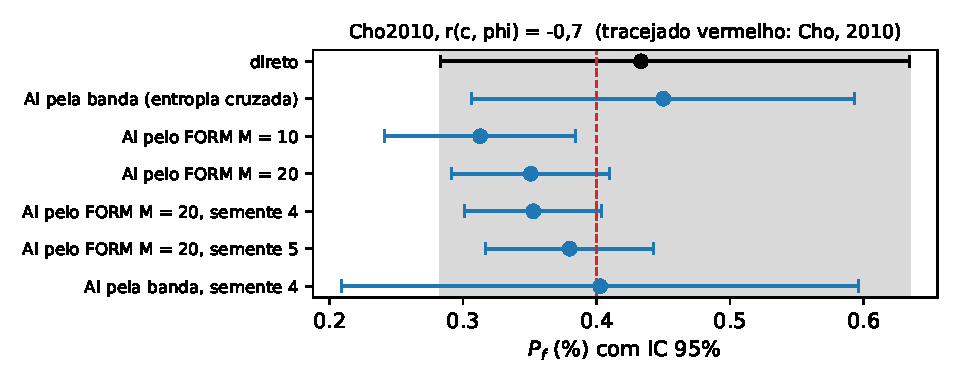
\includegraphics[width=0.85\textwidth]{figs/pf_r07.pdf}
\caption{$P_f$ e IC 95\,\% com $r = -0{,}7$.}\end{figure}

\subsection*{Um modo de ruptura só?}
Se houvesse um segundo mecanismo, a AI pelo FORM quase não o sortearia, e a $P_f$ sairia baixa, com um CoV pequeno enganoso.
Para verificar, os $\bm\xi$ das realizações do direto foram sorteados de novo, sem elementos finitos, com o modo
\texttt{linear} do Cho2010. Em cada realização calculou-se $t = \bm\alpha\cdot\bm\xi$, a coordenada na direção do ponto de
projeto do FORM ($M = 20$).
\begin{itemize}
  \item \textbf{Direção:} nenhuma falha tem $t < 1$. O menor $t$ entre as falhas é 1{,}31 com $r = -0{,}5$ (408 falhas) e 2{,}20 com $r = -0{,}7$ (93 falhas).
  \item \textbf{Geometria:} a banda de ruptura das falhas é a mesma no direto e nas AI ponderadas: profundidade de
    3{,}7\,m e centro em $x \approx 16{,}6$\,m.
  \item \textbf{Conclusão:} há um modo só. Os desvios negativos da AI pelo FORM (de $-0{,}6$ a $-1{,}3$) são compatíveis com o
    acaso. As duas AI de cada $r$ usam a mesma semente e não são independentes. As repetições com sementes novas
    (\texttt{\_s4}, \texttt{\_s5}) vão confirmar.
\end{itemize}
\begin{figure}[H]\centering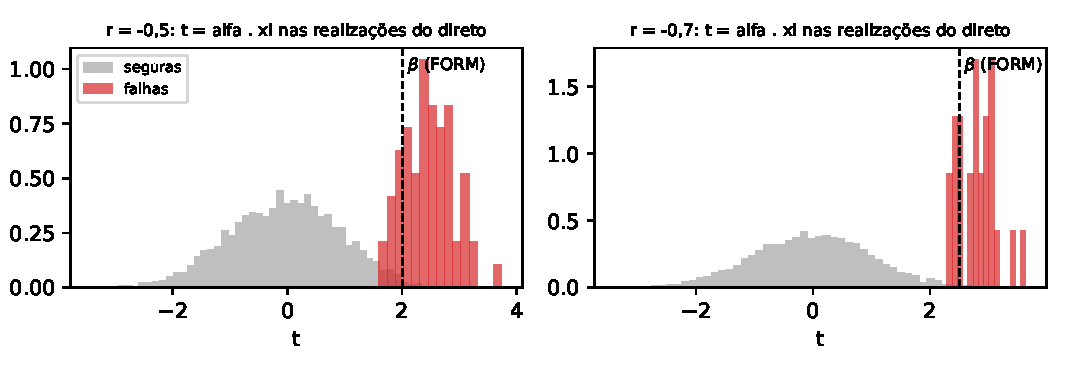
\includegraphics[width=\textwidth]{figs/modo.pdf}
\caption{$t = \bm\alpha\cdot\bm\xi$ nas realizações do direto. As falhas (vermelho) ficam todas à direita, perto ou além de
$\beta$.}\end{figure}

\section{Pós-processamento}
\subsection*{Tamanho do piloto (AI pela banda)}
O deslocamento da AI pela banda é $\bm\mu = s_c\,\bm d_c + s_\varphi\,\bm d_\varphi$, com $s$ = a média de $\bm\xi\cdot\bm d$ no
conjunto elite do piloto (os 10\,\% de menor FS, ou as falhas se forem mais). Para ver quanto $s$ depende do tamanho do
piloto, o direto foi dividido em sub-pilotos disjuntos de 100, 250, 500 e 1000 realizações. As projeções foram refeitas
sem elementos finitos, pelo modo \texttt{linear} com \texttt{banda=}. O sub-piloto 0--999 reproduz o deslocamento que o
programa usou no fermi: $s = (-0{,}479; -1{,}367)$.
\begin{table}[H]\centering\small
\resizebox{\textwidth}{!}{%
\begin{tabular}{lrrrrr}
\toprule
caso & piloto & sub-pilotos & $s_c$: média (dp) & $s_\varphi$: média (dp) & $|\bm\mu|^2$: média (dp) \\
\midrule
$r = -0{,}5$ & 100 & 40 & -0{,}31 (0{,}29) & -1{,}32 (0{,}24) & 1{,}99 (0{,}63) \\
$r = -0{,}5$ & 250 & 16 & -0{,}33 (0{,}18) & -1{,}35 (0{,}11) & 1{,}96 (0{,}32) \\
$r = -0{,}5$ & 500 & 8 & -0{,}32 (0{,}14) & -1{,}32 (0{,}10) & 1{,}87 (0{,}28) \\
$r = -0{,}5$ & 1000 & 4 & -0{,}32 (0{,}15) & -1{,}34 (0{,}07) & 1{,}92 (0{,}22) \\
$r = -0{,}7$ & 100 & 60 & -0{,}06 (0{,}26) & -1{,}33 (0{,}27) & 1{,}89 (0{,}70) \\
$r = -0{,}7$ & 250 & 24 & -0{,}03 (0{,}17) & -1{,}34 (0{,}14) & 1{,}85 (0{,}39) \\
$r = -0{,}7$ & 500 & 12 & -0{,}03 (0{,}14) & -1{,}34 (0{,}11) & 1{,}83 (0{,}32) \\
$r = -0{,}7$ & 1000 & 6 & -0{,}05 (0{,}12) & -1{,}35 (0{,}07) & 1{,}84 (0{,}19) \\
\bottomrule
\end{tabular}}
\caption{O deslocamento da banda com pilotos de tamanhos diferentes.}
\end{table}
A média de $s$ não depende do tamanho do piloto; só a dispersão cai. Um erro $\bm\delta$ no deslocamento multiplica a
variância da AI por cerca de $e^{|\bm\delta|^2}$. Com piloto de 100, $|\bm\delta|^2 \approx 0{,}14$ (variância $\times1{,}15$); com 250, $0{,}04$ ($\times1{,}05$). Valores com $r = -0{,}5$. Um piloto de 250 basta.

\subsection*{Custo total para CoV$(P_f) = 10\,\%$}
O número de análises para chegar a CoV de 10\,\% é $N\,(\mathrm{CoV}/0{,}10)^2$. A ele soma-se o custo fixo de cada método:
o piloto de 1000 na banda e as análises do FORM.
\begin{table}[H]\centering\small
\resizebox{\textwidth}{!}{%
\begin{tabular}{lrrrrrr}
\toprule
Método & $r = -0{,}5$: amostragem & + fixo & total & $r = -0{,}7$: amostragem & + fixo & total \\
\midrule
Monte Carlo direto & 5782 & 0 & 5782 & 26782 & 0 & 26782 \\
AI pela banda (entropia cruzada) & 1238 & 1000 & 2238 & 2645 & 1000 & 3645 \\
AI pelo FORM $M = 10$ & 773 & 123 & 896 & 1354 & 164 & 1518 \\
AI pelo FORM $M = 20$ & 396 & 243 & 639 & 741 & 243 & 984 \\
\bottomrule
\end{tabular}}
\caption{Análises de elementos finitos para CoV$(P_f) = 10\,\%$.}
\end{table}
Mesmo pagando o FORM, a AI pelo ponto de projeto custa de 6 a 27 vezes menos que o direto. A vantagem cresce quando a $P_f$ cai. O piloto de
1000 da banda pesa muito. Com um piloto de 250, que basta (tabela anterior), a banda iria a 1488 e 2895 análises, ainda 1,5 a 3 vezes o FORM.

\subsection*{A previsão teórica: $M = 10$ contra $M = 20$}
No modelo linear, deslocar para o ponto de projeto truncado multiplica a variância da AI por cerca de
$\exp(\beta_{10}^2 - \beta_{20}^2)$. As duas AI de cada $r$ usam a mesma semente (números aleatórios comuns).
\begin{table}[H]\centering\small
\resizebox{\textwidth}{!}{%
\begin{tabular}{lrr}
\toprule
caso & previsto: $\exp(\beta_{10}^2-\beta_{20}^2)$ & medido: $(\mathrm{CoV}_{10}/\mathrm{CoV}_{20})^2$ \\
\midrule
$r = -0{,}5$ & 1{,}53 & 1{,}95 \\
$r = -0{,}7$ & 1{,}99 & 1{,}83 \\
\bottomrule
\end{tabular}}
\caption{A razão das variâncias das AI com o ponto de projeto de $M = 10$ e de $M = 20$.}
\end{table}
A ordem de grandeza confere: o $M = 20$ reduz a variância à metade. Com 1000 amostras, o próprio CoV tem cerca de 10\,\% de
erro, e as razões medidas são compatíveis com as previstas.

\section{Etapa 4: a referência da chuva}
O caso é o f50 de Rahardjo a 31,05\,mm/h, com o FS só em 24\,h.
\begin{table}[H]\centering\small
\resizebox{\textwidth}{!}{%
\begin{tabular}{lrrrrrrr}
\toprule
Método & $N$ & $P_f$ (\%) & IC 95\% (\%) & CoV (\%) & dif. (desvios) & ESS$_F$ & ganho \\
\midrule
Monte Carlo direto & 9093 & 5{,}45 & 5{,}00–5{,}94 & 4{,}4 & --- & --- & 1 \\
AI pela banda, semente 1 & 1000 & 6{,}18 & 5{,}33–7{,}03 & 7{,}0 & 1{,}5 & 168 & 3{,}1 \\
AI pela banda, semente 2 & 1000 & 5{,}74 & 4{,}82–6{,}66 & 8{,}2 & 0{,}5 & 130 & 2{,}4 \\
\bottomrule
\end{tabular}}
\caption{Chuva: o Monte Carlo direto de 4000 é a referência para validar o FORM e a AI na chuva (etapa 4).}
\end{table}
A AI pela banda concorda com o direto (1{,}5 desvio), com ganho de 3{,}1$\times$. Falta o FORM na chuva, que precisa de código novo (as opções \texttt{M},
\texttt{xi} e \texttt{desloc\_xi} no \texttt{montecarlo.cpp}).

\section{Próximos passos}
\begin{enumerate}
  \item Juntar as repetições independentes da AI, que estão rodando no fermi, e fechar a questão do pequeno desvio da AI pelo
    FORM.
  \item Etapa 4: o código do FORM e da AI pelo ponto de projeto na chuva, validados contra o direto de 4000.
  \item Para o artigo da AI: a AI pelo FORM $M = 20$ deu o maior ganho (até 51$\times$ com $P_f \approx 0{,}4\,\%$), contando só a amostragem. O custo do FORM é de 243 análises. Mesmo somando
    esse custo, ele ainda vence a AI pela banda, que precisa de um piloto de 1000.
\end{enumerate}
\end{document}
